
 
\documentclass[a4paper,12pt]{article} % This defines the style of your paper

% We usually use the article type. The additional parameters are the format of the paper you want to print it on and the standard font size. For us this is a4paper and 12pt.

%%%%%%%%%%%%%%%%%%%%%%%%%%%%%%%%%%%%%%%%%%%%%%%%
% 2. Packages
%%%%%%%%%%%%%%%%%%%%%%%%%%%%%%%%%%%%%%%%%%%%%%%%

% Packages are libraries of commands that LaTeX can call when compiling the document. With the specialized commands you can customize the formatting of your document.
% If the packages we call are not installed yet, TeXworks will ask you to install the necessary packages while compiling.

% First, we usually want to set the margins of our document. For this we use the package geometry. We call the package with the \usepackage command. The package goes in the {}, the parameters again go into the [].
\usepackage[top = 2.5cm, bottom = 2.5cm, left = 2.5cm, right = 2.5cm]{geometry} 

% Unfortunately, LaTeX has a hard time interpreting German Umlaute. The following two lines and packages should help. If it doesn't work for you please let me know.
\usepackage[T1]{fontenc}
\usepackage[utf8]{inputenc}


% The following two packages - multirow and booktabs - are needed to create nice looking tables.
\usepackage{multirow} % Multirow is for tables with multiple rows within one cell.
\usepackage{booktabs} % For even nicer tables.

% As we usually want to include some plots (.pdf files) we need a package for that.
\usepackage{graphicx} 
\usepackage[export]{adjustbox}
\usepackage{caption}
\usepackage{wrapfig}
\usepackage{listings}
\usepackage{courier}

\lstset{basicstyle=\footnotesize\ttfamily,breaklines=true}
\lstset{framextopmargin=50pt}
\usepackage{hyperref}


% The default setting of LaTeX is to indent new paragraphs. This is useful for articles. But not really nice for homework problem sets. The following command sets the indent to 0.
\usepackage{setspace}
\setlength{\parindent}{0in}

% Package to place figures where you want them.
\usepackage{float}

% The fancyhdr package let's us create nice headers.
\usepackage{fancyhdr}

\usepackage{biblatex}
\addbibresource{geo1001.bib}


%%%%%%%%%%%%%%%%%%%%%%%%%%%%%%%%%%%%%%%%%%%%%%%%
% 3. Header (and Footer)
%%%%%%%%%%%%%%%%%%%%%%%%%%%%%%%%%%%%%%%%%%%%%%%%

% To make our document nice we want a header and number the pages in the footer.

\pagestyle{fancy} % With this command we can customize the header style.

\fancyhf{} % This makes sure we do not have other information in our header or footer.

\lhead{\footnotesize GEO1001: Homework 1}% \lhead puts text in the top left corner. \footnotesize sets our font to a smaller size.

%\rhead works just like \lhead (you can also use \chead)
\rhead{\footnotesize Michiel de Jong (4376978)} %<---- Fill in your lastnames.

% Similar commands work for the footer (\lfoot, \cfoot and \rfoot).
% We want to put our page number in the center.
\cfoot{\footnotesize \thepage} 


%%%%%%%%%%%%%%%%%%%%%%%%%%%%%%%%%%%%%%%%%%%%%%%%
% 4. Your document
%%%%%%%%%%%%%%%%%%%%%%%%%%%%%%%%%%%%%%%%%%%%%%%%

% Now, you need to tell LaTeX where your document starts. We do this with the \begin{document} command.
% Like brackets every \begin{} command needs a corresponding \end{} command. We come back to this later.

\begin{document}


%%%%%%%%%%%%%%%%%%%%%%%%%%%%%%%%%%%%%%%%%%%%%%%%
%%%%%%%%%%%%%%%%%%%%%%%%%%%%%%%%%%%%%%%%%%%%%%%%

%%%%%%%%%%%%%%%%%%%%%%%%%%%%%%%%%%%%%%%%%%%%%%%%
% Title section of the document
%%%%%%%%%%%%%%%%%%%%%%%%%%%%%%%%%%%%%%%%%%%%%%%%

% For the title section we want to reproduce the title section of the Problem Set and add your names.

\thispagestyle{empty} % This command disables the header on the first page. 

\begin{tabular}{p{15.5cm}} % This is a simple tabular environment to align your text nicely 
{\large \bf Sensing Technologies and Mathematics for Geomatics} \\
GEO1001.2020 \\ MSc Geomatics \\ Delft University of Technology \\
\hline % \hline produces horizontal lines.
\\
\end{tabular} % Our tabular environment ends here.

\vspace*{0.3cm} % Now we want to add some vertical space in between the line and our title.

\begin{center} % Everything within the center environment is centered.
	{\Large \bf Homework 1} % <---- Don't forget to put in the right number
	\vspace{2mm}
	
        % YOUR NAMES GO HERE
	{\bf Michiel de Jong (4376978)} % <---- Fill in your names here!
		
\end{center}  

\vspace{0.4cm}

%%%%%%%%%%%%%%%%%%%%%%%%%%%%%%%%%%%%%%%%%%%%%%%%
%%%%%%%%%%%%%%%%%%%%%%%%%%%%%%%%%%%%%%%%%%%%%%%%

% Up until this point you only have to make minor changes for every week (Number of the homework). Your write up essentially starts here.
For the first homework, we have to analyse data \cite{Maiullari2020} from 5 Kestrel sensors. Throughout this report, we will see the results from this analysis. The analysis has been done using Python. A complete repository for the project can be found on: \url{https://github.com/dumigil/geo1001_hw01 }

\begin{enumerate}

\item {\it Compute mean statistics (mean, variance and standard deviation for each of the sensors variables), what do you observe from the results?}. % <--- For future Homework sets you of course have to change the questions.

% Please add the following required packages to your document preamble:
% \usepackage{graphicx}
\begin{table}[H]
\centering
\resizebox{\textwidth}{!}{%
\begin{tabular}{|l|l|l|l|l|l|l|l|l|l|l|l|l|l|l|l|}
 & \multicolumn{5}{l|}{Mean} & \multicolumn{5}{l|}{STD} & \multicolumn{5}{l|}{Var} \\ \hline
 & A & B & C & D & E & A & B & C & D & E & A & B & C & D & E \\ \hline
Direction\_True & 209,406 & 183,412 & 183,589 & 198,327 & 223,956 & 100,543 & 99,886 & 87,769 & 90,188 & 96,479 & 10108,940 & 9977,218 & 7703,363 & 8133,890 & 9308,285 \\
Wind\_Speed & 1,290 & 1,242 & 1,371 & 1,582 & 0,596 & 1,119 & 1,141 & 1,196 & 1,319 & 0,715 & 1,251 & 1,302 & 1,431 & 1,740 & 0,511 \\
Crosswind\_Speed & 0,965 & 0,836 & 0,963 & 1,211 & 0,439 & 0,963 & 0,937 & 1,021 & 1,205 & 0,562 & 0,927 & 0,879 & 1,043 & 1,452 & 0,316 \\
Headwind\_Speed & 0,164 & -0,130 & -0,263 & -0,301 & 0,195 & 1,017 & 1,121 & 1,128 & 1,110 & 0,565 & 1,035 & 1,257 & 1,272 & 1,233 & 0,319 \\
Temperature & 17,969 & 18,065 & 17,913 & 17,996 & 18,354 & 3,983 & 4,078 & 4,013 & 4,013 & 4,364 & 15,864 & 16,629 & 16,105 & 16,106 & 19,043 \\
Globe\_Temperature & 21,545 & 21,799 & 21,587 & 21,359 & 21,176 & 8,258 & 8,127 & 8,243 & 7,823 & 7,951 & 68,191 & 66,049 & 67,941 & 61,202 & 63,216 \\
Wind\_Chill & 17,838 & 17,946 & 17,773 & 17,835 & 18,294 & 4,033 & 4,127 & 4,067 & 4,069 & 4,375 & 16,264 & 17,036 & 16,541 & 16,557 & 19,137 \\
Relative\_Humidity & 78,185 & 77,878 & 77,963 & 77,942 & 76,793 & 19,391 & 20,214 & 19,355 & 19,745 & 20,162 & 376,010 & 408,623 & 374,623 & 389,856 & 406,494 \\
Heat\_Stress\_Index & 17,900 & 18,004 & 17,828 & 17,922 & 18,286 & 3,873 & 3,929 & 3,919 & 3,888 & 4,298 & 14,997 & 15,439 & 15,356 & 15,118 & 18,475 \\
Dew\_Point & 13,554 & 13,531 & 13,458 & 13,509 & 13,559 & 3,118 & 3,104 & 3,176 & 3,174 & 3,070 & 9,723 & 9,637 & 10,084 & 10,072 & 9,423 \\
Psychro\_WBT & 15,271 & 15,296 & 15,197 & 15,260 & 15,407 & 2,635 & 2,602 & 2,691 & 2,654 & 2,645 & 6,944 & 6,770 & 7,239 & 7,044 & 6,997 \\
Station\_Pressure & 1016,168 & 1016,657 & 1016,689 & 1016,728 & 1016,166 & 6,203 & 6,070 & 6,139 & 5,915 & 6,240 & 38,471 & 36,842 & 37,691 & 34,988 & 38,940 \\
Barometric\_Pressure & 1016,128 & 1016,616 & 1016,652 & 1016,689 & 1016,128 & 6,202 & 6,069 & 6,138 & 5,912 & 6,240 & 38,468 & 36,829 & 37,676 & 34,952 & 38,935 \\
Altitude & -25,987 & -30,058 & -30,339 & -30,653 & -25,961 & 51,610 & 50,455 & 51,074 & 49,191 & 51,888 & 2663,641 & 2545,708 & 2608,535 & 2419,724 & 2692,353 \\
Density\_Altitude & 137,317 & 135,581 & 129,623 & 132,411 & 150,840 & 162,819 & 163,900 & 164,276 & 162,838 & 172,380 & 26510,044 & 26863,310 & 26986,603 & 26516,126 & 29714,928 \\
NA\_WBT & 15,982 & 15,997 & 15,934 & 15,916 & 15,937 & 3,164 & 3,132 & 3,237 & 3,160 & 3,071 & 10,012 & 9,809 & 10,480 & 9,987 & 9,432 \\
WBGT & 17,254 & 17,322 & 17,225 & 17,177 & 17,186 & 4,017 & 3,979 & 4,068 & 3,938 & 3,936 & 16,135 & 15,835 & 16,547 & 15,507 & 15,490 \\
TWL & 301,393 & 299,452 & 301,900 & 305,255 & 284,115 & 28,544 & 28,108 & 27,686 & 24,820 & 35,915 & 814,767 & 790,069 & 766,534 & 616,010 & 1289,913 \\
Direction\_Mag & 208,905 & 183,217 & 183,084 & 197,826 & 223,897 & 100,527 & 99,877 & 87,776 & 90,196 & 96,270 & 10105,677 & 9975,447 & 7704,620 & 8135,316 & 9268,008 \\ \hline
\end{tabular}%
}
\caption{\label{tab:table-name}Mean, Standard Deviation and Variance for all data.}
\end{table}
On first glance, the mean values in the table seem to vary quite a bit per sensor, though we cannot say if this is statistically significant. However, it could be an indication that we can gather some good information from these five sensors.  The standard deviation values show consistent values across the five sensors. The standard deviation for values related to pressure, which generally does not vary a lot during a day, show a low value consistent with this behaviour, while values related to temperature (which can vary a lot during the day) show much higher standard deviations.  
The variance, which is the standard deviation squared (actually the other way around), shows values consistent with this mathematical relationship.   
\item {\it Create 1 plot that contains histograms for the 5 sensors Temperature values. Compare histograms with 5 and 50 bins, why is the number of bins important?}

When comparing the figures below, we can see that although the general shapes of the histograms are rather similar, a lot of information is lost when using only 5 bins. Too many bins however, are also not ideal, as this can cause interference. There are some guidelines to determine the number of bins for a histogram, such as Rice's rule. If we apply Rice's rule to this sample, with Rice's rule being defined as: $k = 2 * \sqrt[3]{n}$. With n being approximately 2500 for all sensors, we thus get $2* \sqrt[3]{2500} = 27.144$, which would give us 27 bins. This is the number of bins used for histograms and histogram derived plots in this assignment.

\begin{figure}[H]
  \centering
  \begin{minipage}[b]{0.45\textwidth}
    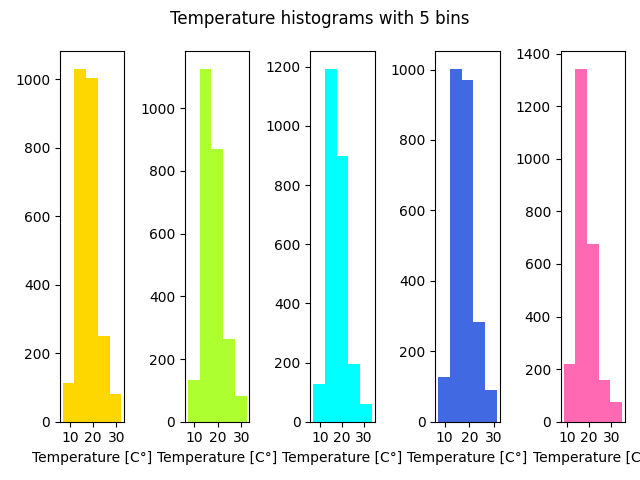
\includegraphics[width=\textwidth]{plot_temps_hist_5.png}
    \caption{Histogram of five sensors using 5 bins}
  \end{minipage}
  \hfill
  \begin{minipage}[b]{0.45\textwidth}
    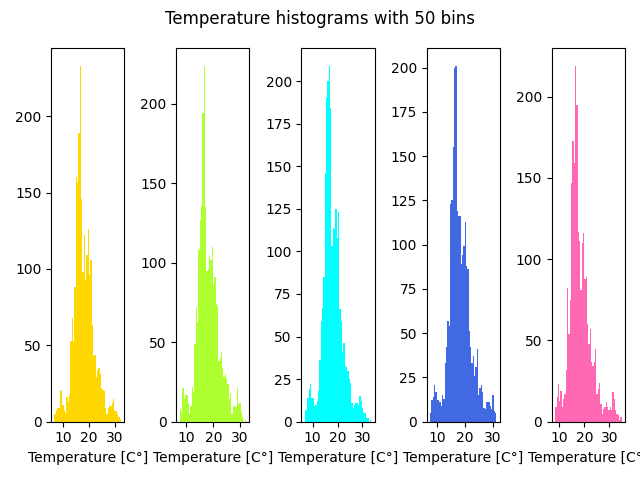
\includegraphics[width=\textwidth]{plot_temps_hist_50.png}
    \caption{Histogram of five sensors using 50 bins}
  \end{minipage}
\end{figure}

\item {\it Create 1 plot where frequency polygons for the 5 sensors Temperature values overlap in different colors with a legend.}
 \begin{figure}[H] % places figure environment here   
    \centering % Centers Graphic
    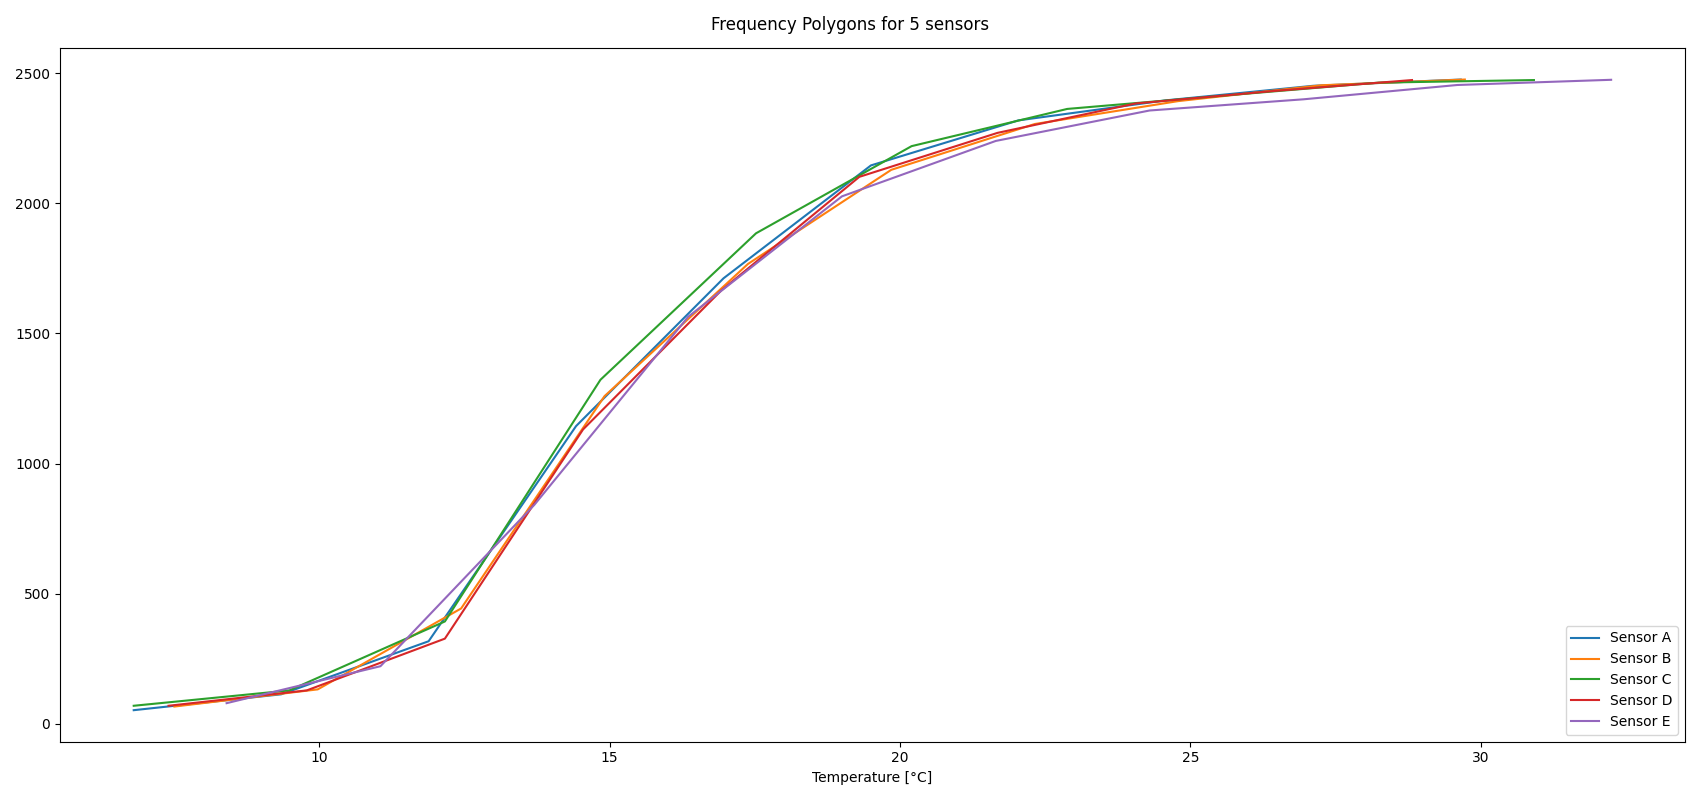
\includegraphics[width=0.9\textwidth]{frequency_polygon.png} 
    \caption{Frequency polygons for the 5 sensors Temperature values} % Creates caption underneath graph
  \end{figure}
In the figure above, we see that the five sensors have similar frequency polygons. From this we could infer, that they have similar distributions, which would support the observation we already made by looking at the histograms in the previous question. 
\newpage
\item {\it Generate 3 plots that include the 5 sensors box plot for: Wind Speed, Wind Direction and Temperature.}
\begin{figure}[H] % places figure environment here   
    \centering % Centers Graphic
    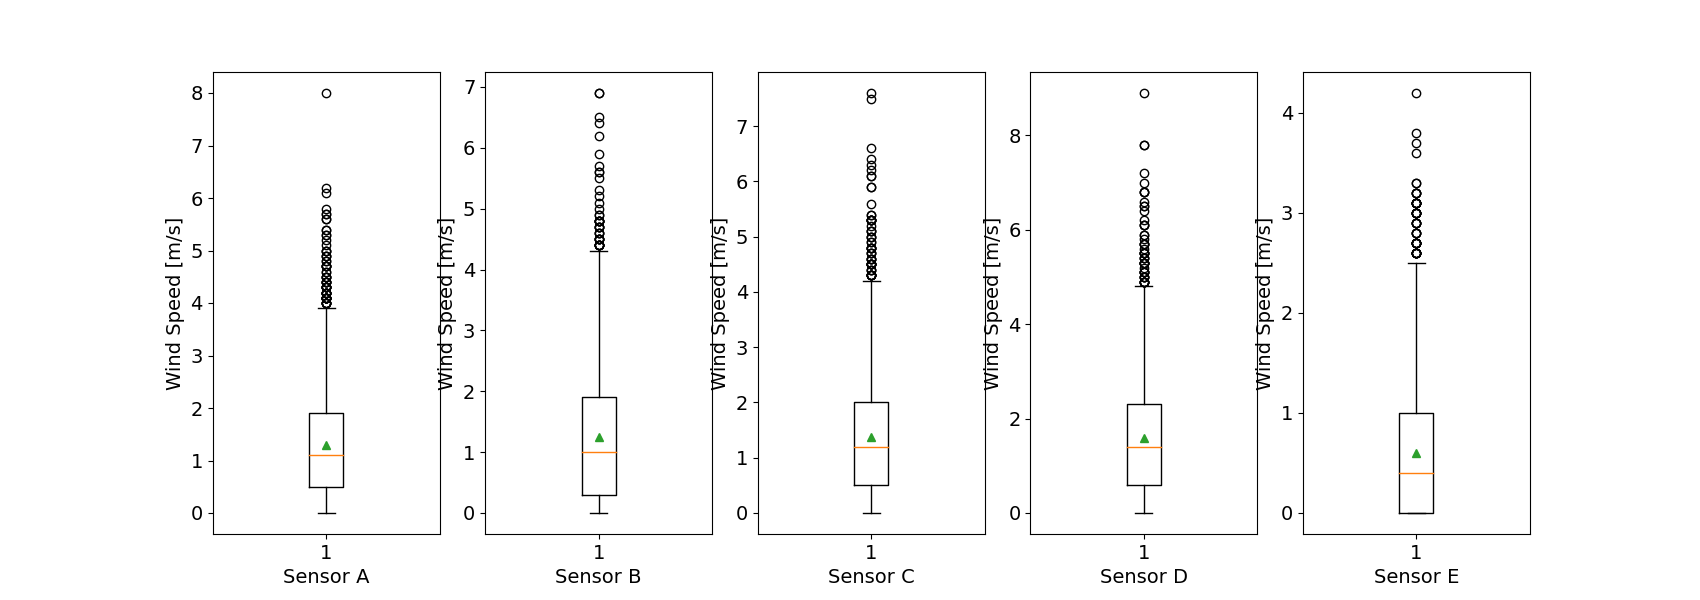
\includegraphics[width=0.9\textwidth]{boxplot_windspeed.png} 
    \caption{Box plots for the 5 sensors Wind Speed values} % Creates caption underneath graph
  \end{figure}
\begin{figure}[H] % places figure environment here   
    \centering % Centers Graphic
    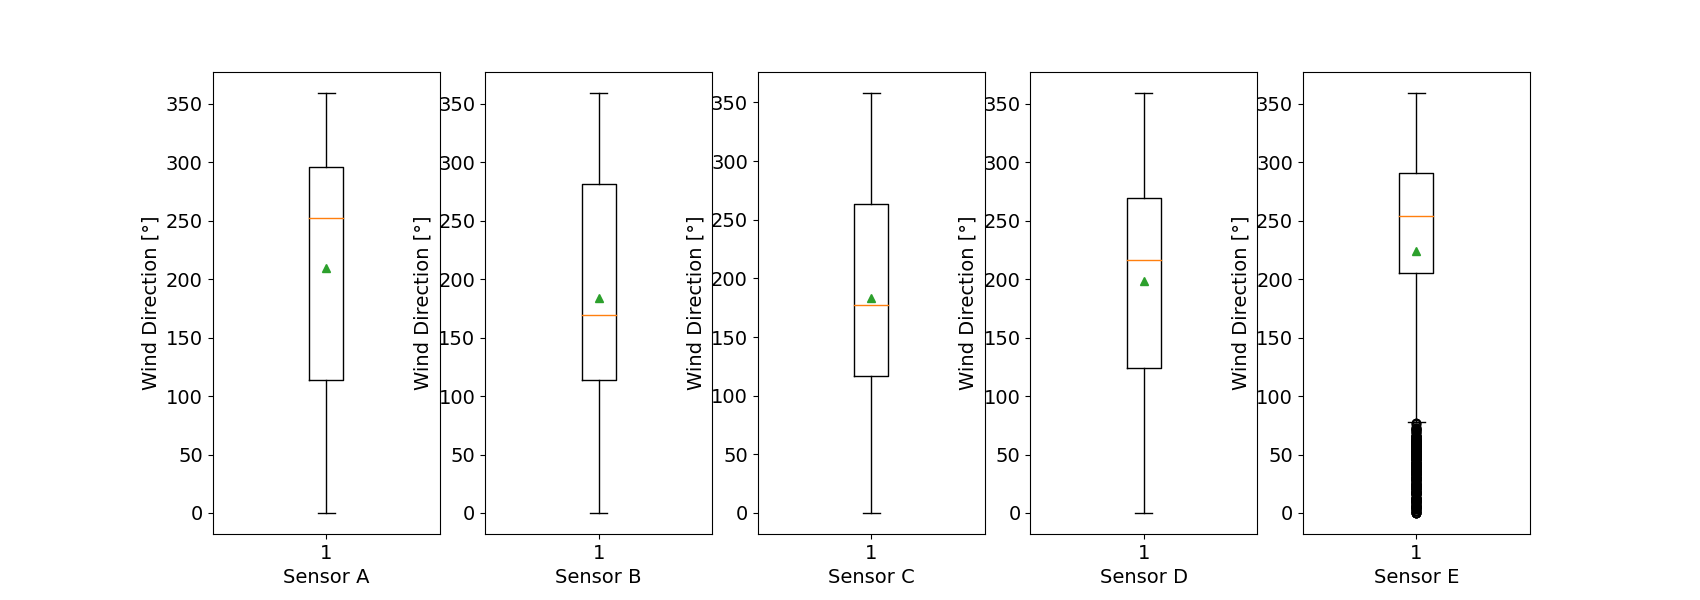
\includegraphics[width=0.9\textwidth]{boxplot_winddirection.png} 
    \caption{Box plots for the 5 sensors Wind Direction values} % Creates caption underneath graph
  \end{figure}
\begin{figure}[H] % places figure environment here   
    \centering % Centers Graphic
    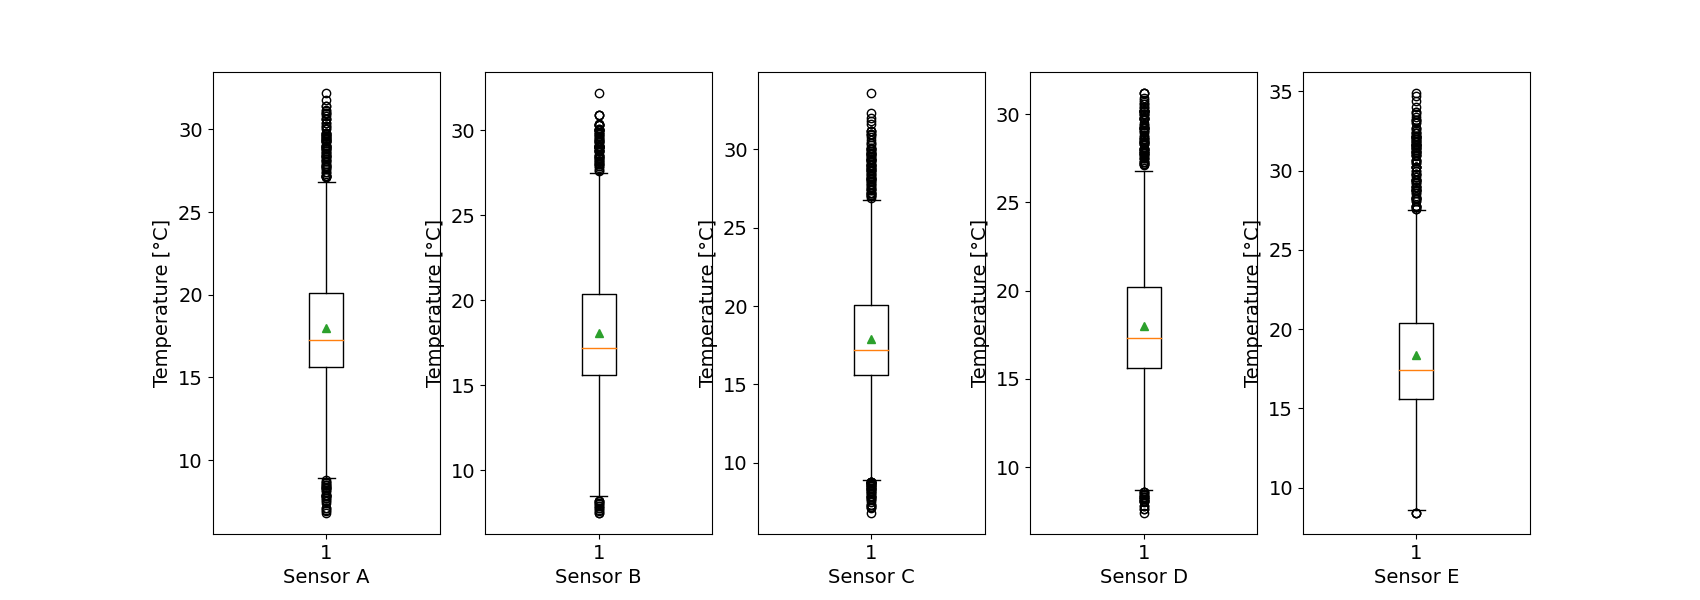
\includegraphics[width=0.9\textwidth]{boxplot_temperature.png} 
    \caption{Box plots for the 5 sensors Temperature values} % Creates caption underneath graph
  \end{figure}
\newpage    
  
\item{\it Plot PMF, PDF and CDF for the 5 sensors Temperature values in independent plots (or subplots). Describe the behaviour of the distributions, are they all similar? What about their tails?}
\begin{figure}[H] % places figure environment here   
    \centering % Centers Graphic
    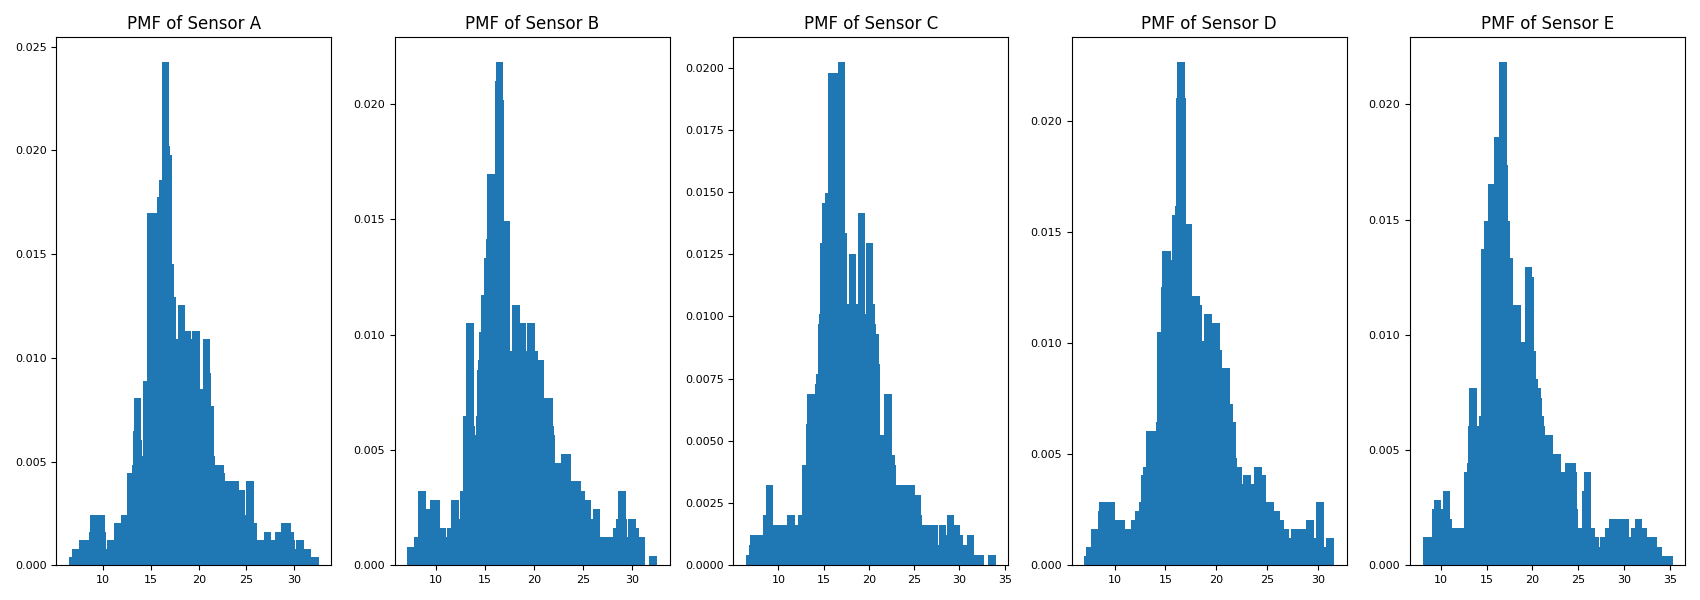
\includegraphics[width=0.9\textwidth]{plot_PMF_T.png} 
    \caption{Probability mass function for the 5 sensors Temperature values} % Creates caption underneath graph
  \end{figure}
  \begin{figure}[H] % places figure environment here   
    \centering % Centers Graphic
    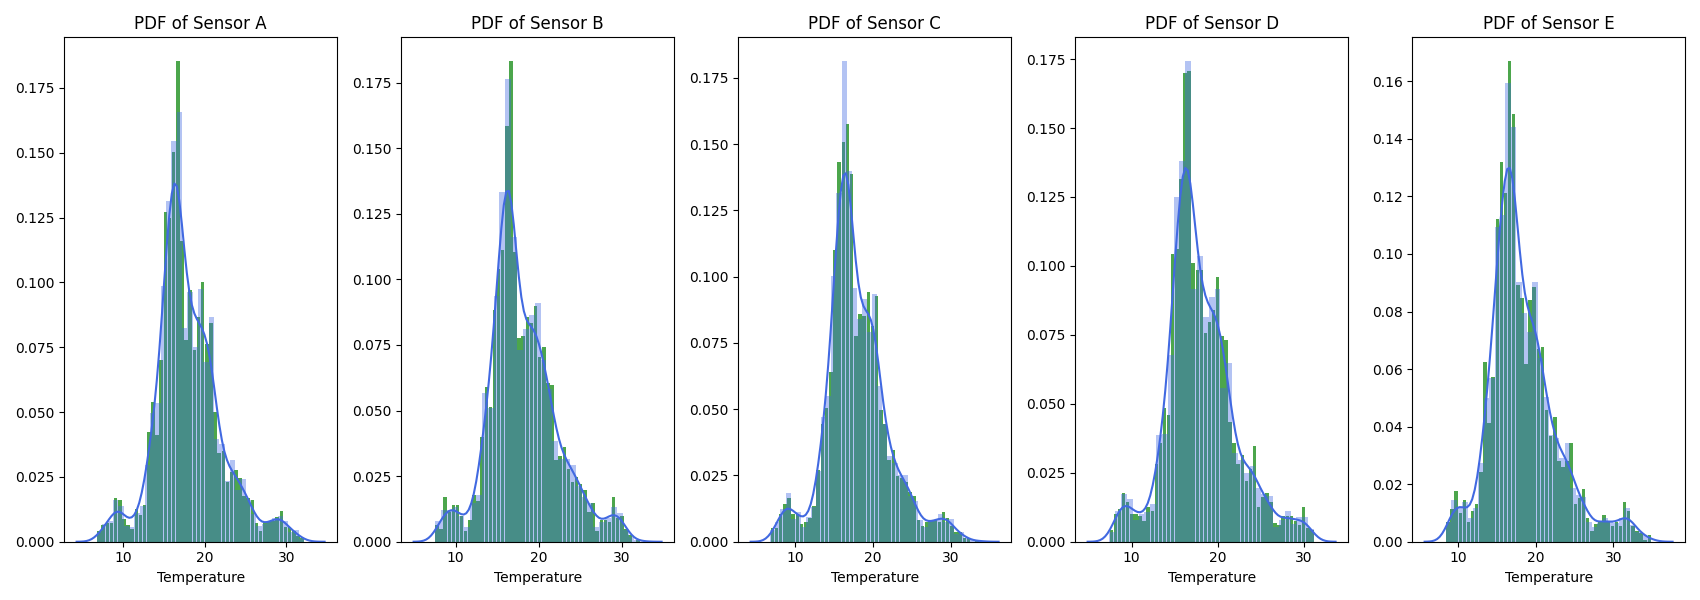
\includegraphics[width=0.9\textwidth]{plot_PDF_T.png} 
    \caption{Probability density function for the 5 sensors Temperature values} % Creates caption underneath graph
  \end{figure}
  \begin{figure}[H] % places figure environment here   
    \centering % Centers Graphic
    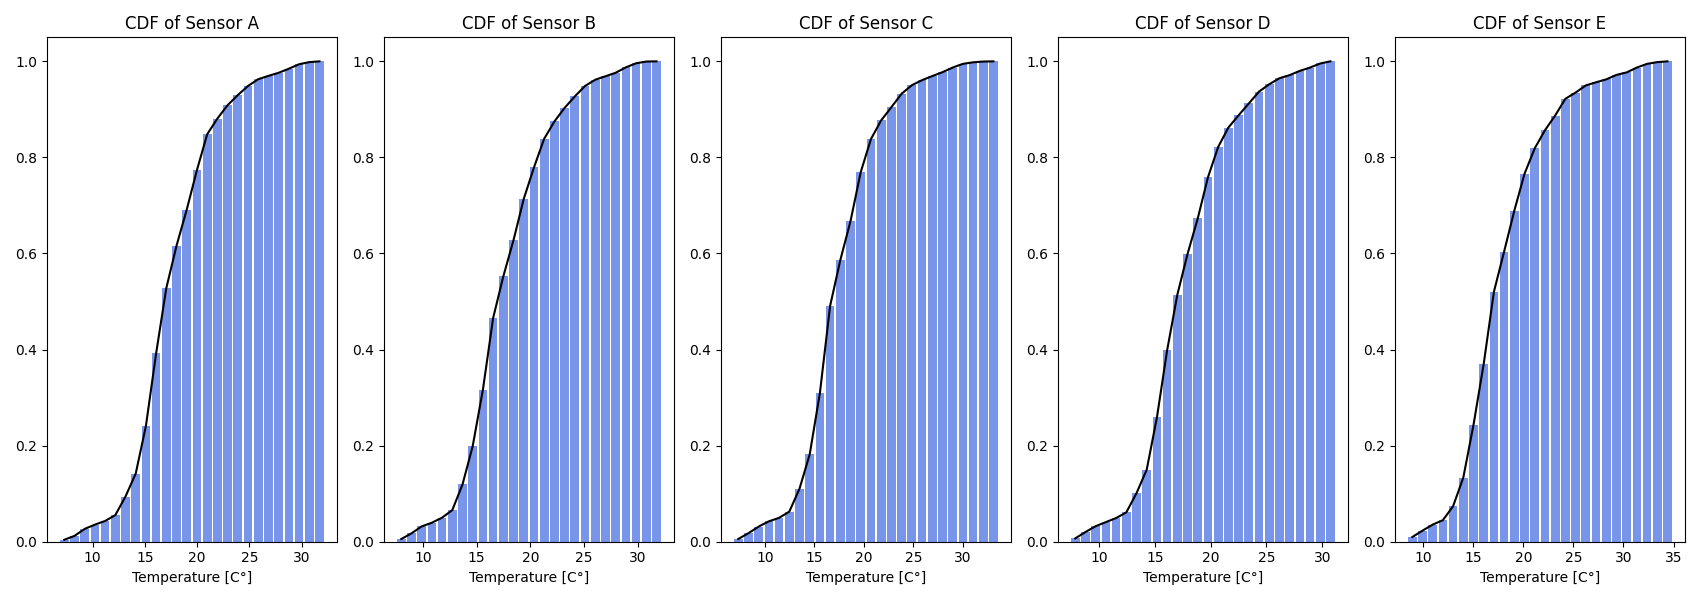
\includegraphics[width=0.9\textwidth]{plot_CDF_T.png} 
    \caption{Cumulative density function for the 5 sensors Temperature values} % Creates caption underneath graph
  \end{figure}
Upon first glance, the PMF and PDF plots look very similar for the five sensors: all five they seem very narrow bell curves, meaning that a lot of the values are centered around the mean. In terms of skewness, all the sensors seem to be skewed slightly to the left, with their peaks around 17-18 degrees celsius. The also have a second mini peak around 20 degrees celsius. This peak is not present left of the mean, which is an interesting observation. All five sensors have a distinct "mini-peak" in both their tails. In terms of kurtosis, the data seems to present narrow peaks, and fatter tails; indicating high kurtosis. When we look back at table 1, we see that all five sensors have similar standard deviation and variance, indicating similar variability. 
\\When looking at the CDF plots, we see our hunch supported, with seeing a higher mass under 0.5 than above it. 
\item{\it For the Wind Speed values, plot the pdf and the kernel density estimation. Comment the differences.}
\begin{figure}[H] % places figure environment here   
    \centering % Centers Graphic
    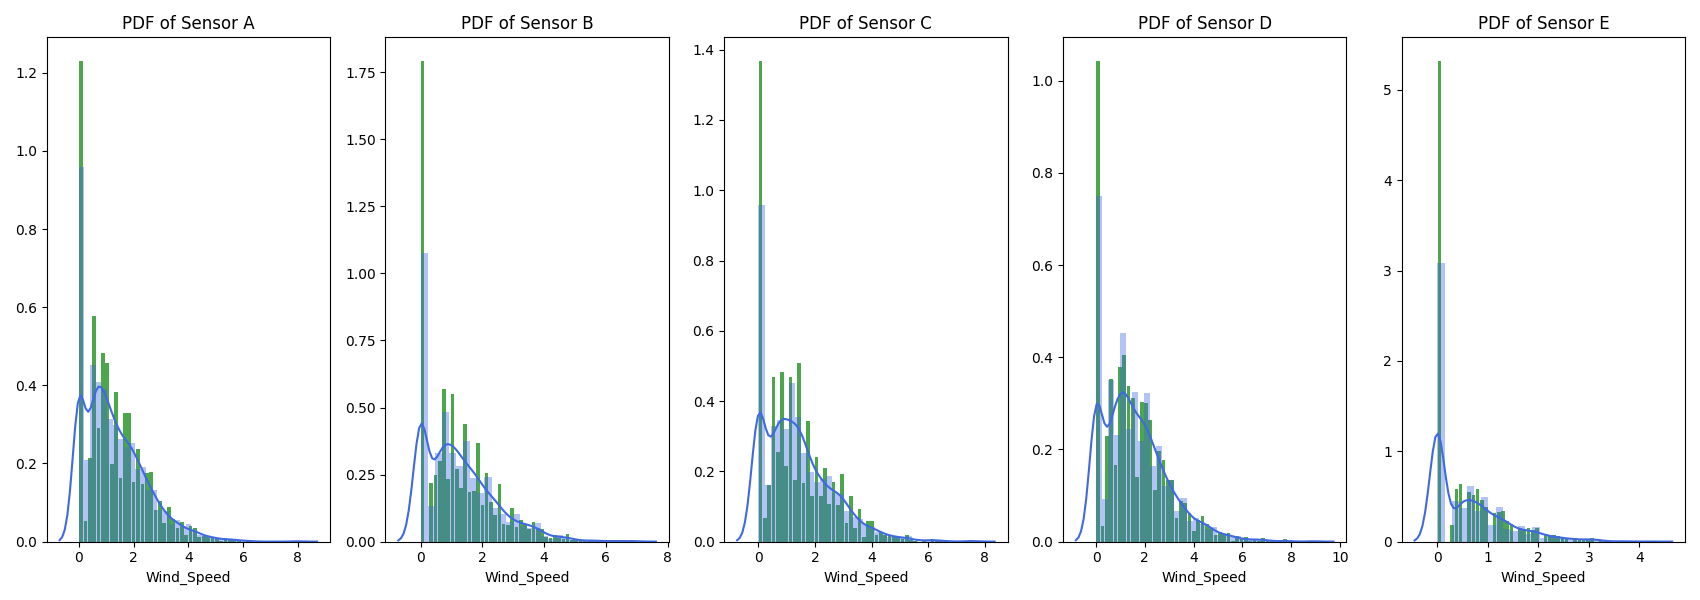
\includegraphics[width=0.9\textwidth]{plot_PDF_WS.png} 
    \caption{Probability density functions for the sensors' Wind Speed measurements.} % Creates caption underneath graph
  \end{figure}
\begin{figure}[H] % places figure environment here   
    \centering % Centers Graphic
    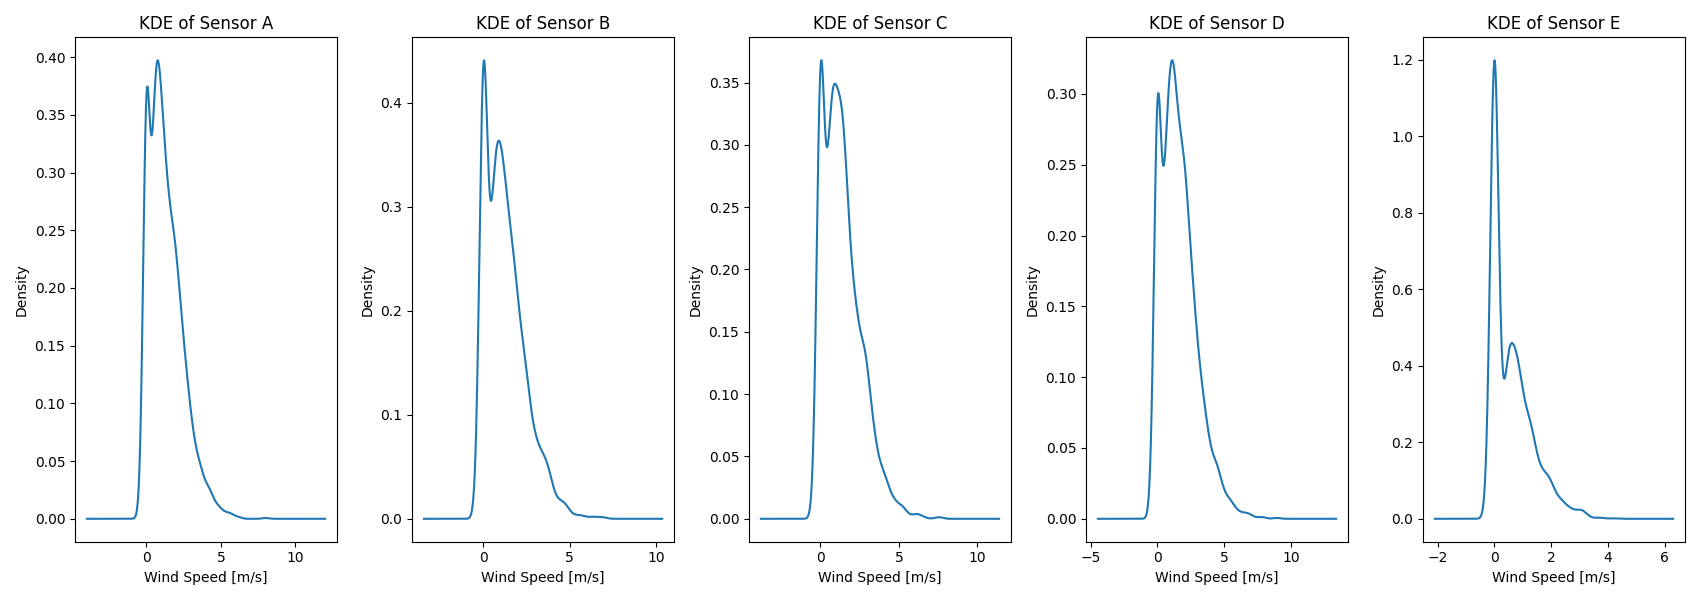
\includegraphics[width=0.9\textwidth]{plot_KDE_WS.png} 
    \caption{Kernel density estimates for the sensors' Wind Speed measurements.} % Creates caption underneath graph
  \end{figure}
The PDF's and the KDE's for Wind Speed differ quite a bit in shape between them. When looking at the PDF's we see that the sensors skew to the right, and have a peak close to zero. Sensors A to D are more similar, with E being the odd one out with a very narrow peak, but also a small tail. This behaviour is translated by the KDE's, which seems to broaden the peak for sensors A to D. In those PDF's we see that there is a second peak around 2 m/s. In sensors A to D, the KDE has tried to combine this peak with the main peak. In sensor E, the proportions observed in the PDF are somewhat maintained.  
\newpage

\item{\it Compute the correlations between all the sensors for the variables: Temperature, Wet Bulb Globe Temperature (WBGT), Crosswind Speed. Perform correlation between sensors with the same variable, not between two different variables; for example, correlate Temperature time series between sensor A and B. Use Pearson’s and Spearman’s rank coefficients. Make a scatter plot with both coefficients with the 3 variables.}
\begin{figure}[H] % places figure environment here   
    \centering % Centers Graphic
    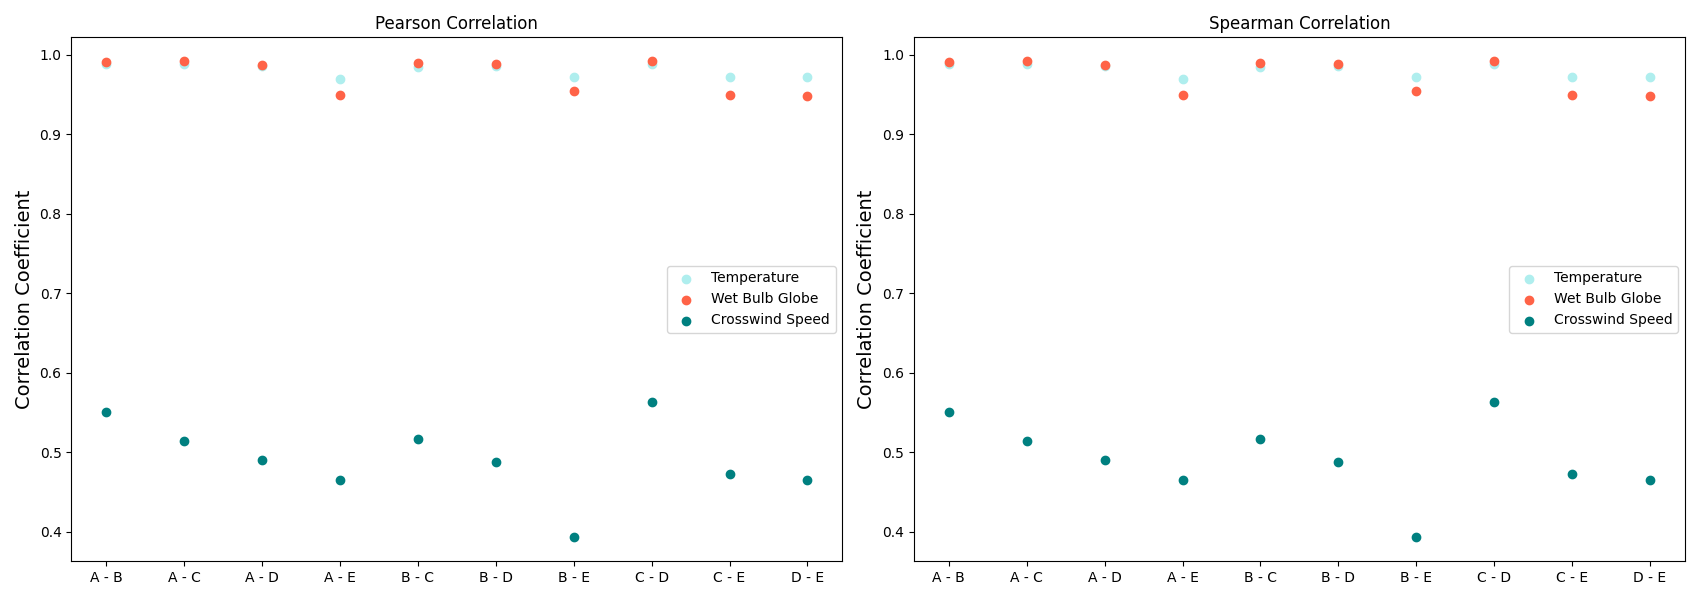
\includegraphics[width=1\textwidth]{plot_correlations.png} 
    \caption{Scatterplot of Pearson and Spearman correlation coefficients for all combinations possible between sensors.} % Creates caption underneath graph
  \end{figure}
\item{\it What can you say about the sensors’ correlations?}
\\When looking at the correlations, we can see that in general, the correlations coefficients for the variables "Temperature" and "Wet Bulb Globe Temperature" are really high, indicating a high level of correlation between the sensors. This makes sense, because they both measure temperature, albeit with slightly different parameters. The correlation coefficients for "Crosswind Speed" vary between 0.4 and 0.6, indicating a lower correlation. However, there is much more variability between the sensors, with stronger correlations in some pairs, and lower correlations in others. 
\newpage
\item{\it If we told you that that the sensors are located as follows, hypothesize which location would you assign to each sensor and reason your hypothesis using the correlations.}
\begin{figure}[H] % places figure environment here   
    \centering % Centers Graphic
    \includegraphics[width=1\textwidth]{sensor_loc.png} 
    \caption{Locations of sensors without labels on a map.} % Creates caption underneath graph
  \end{figure}
We can see that that lowest correlation values for "Temperature" and "WBGT" are A-E, B-E, C-E and D-E, this would suggest that the temperatures at sensor E vary the most from all the other sensors. Thus, I would hypothesize that sensor E will be the sensor in the top right. When looking at the "Wind Speed" correlations, we see that sensor E is also the odd one out. This would further my hypothesis that E is the sensor in the top right, because it looks to be semi enclosed by walls on three sides. 
\\Furthermore, we can see that the correlations for "Cross Wind" between the pairs A-B and C-D are slightly higher than other pairs. This could indicate that A-B are a pair and C-D are a pair, with sensors C and D being in the center open field, and A and B being on the bottom left. C and D both have higher average "Wind Speed" and "Cross Wind Speed" values, which would be consistent with a large open field. By process of elimination, A and B would thus be located bottom left. 
\newpage
\item{\it Plot the CDF for all the sensors and for variables Temperature and Wind Speed, then compute the 95\% confidence intervals for variables Temperature and Wind Speed for all the sensors and save them in a table (txt or csv form).}
\begin{figure}[H] % places figure environment here   
    \centering % Centers Graphic
    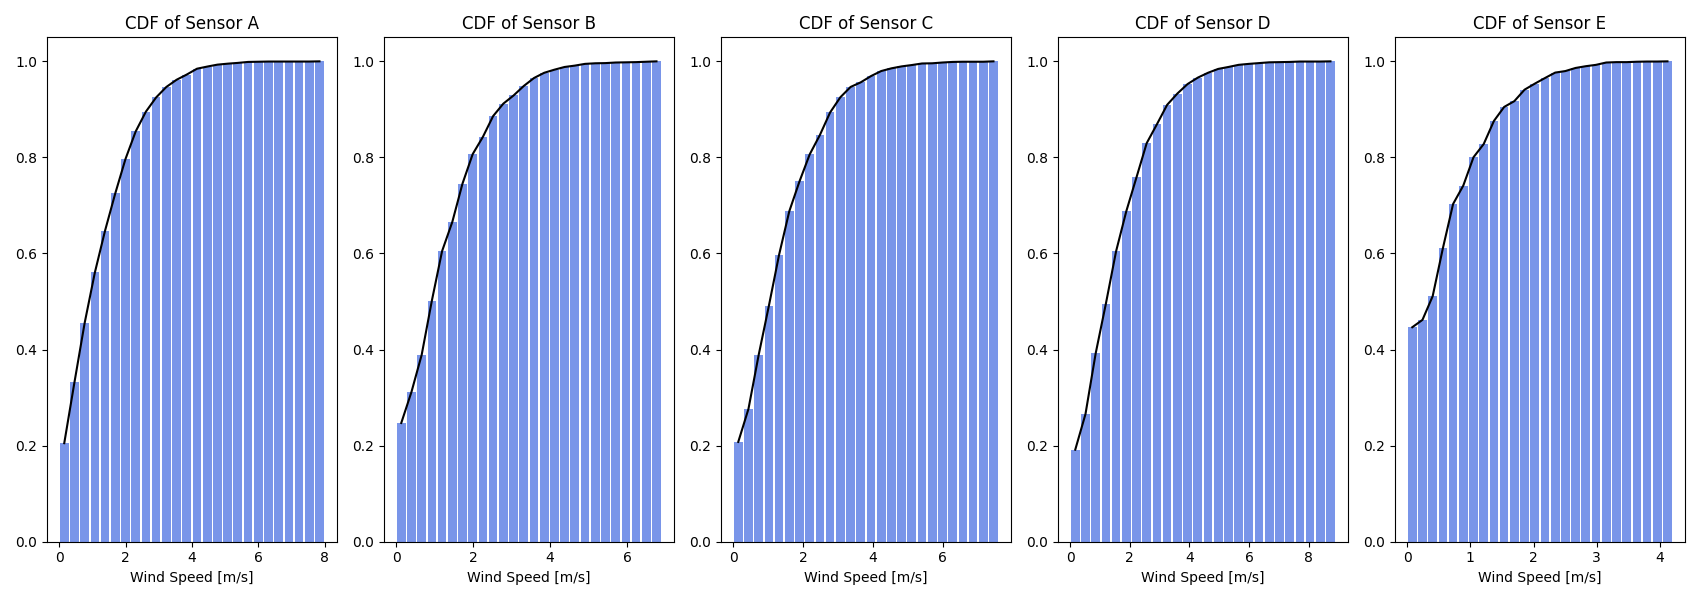
\includegraphics[width=1\textwidth]{plot_CDF_WS.png} 
    \caption{CDF for all the sensors Wind Speed values.} % Creates caption underneath graph
  \end{figure}
  \begin{figure}[H] % places figure environment here   
    \centering % Centers Graphic
    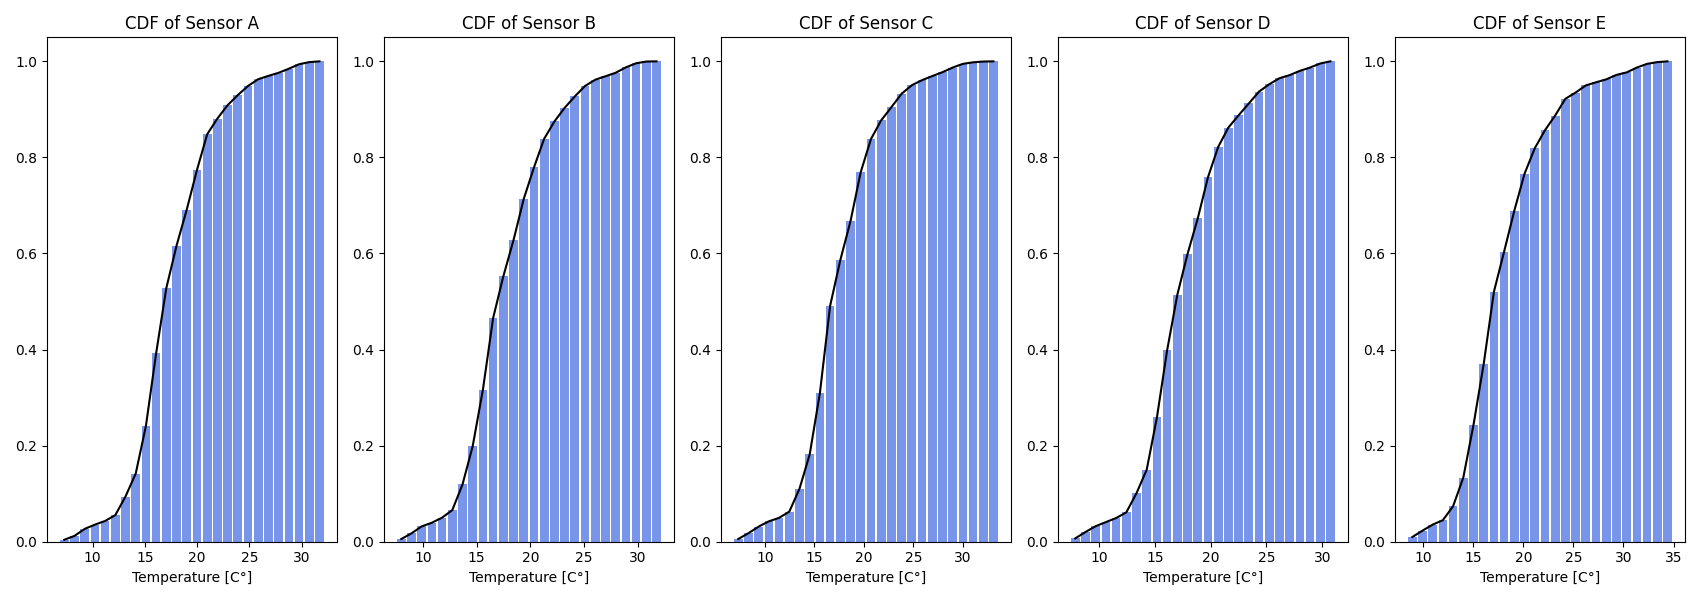
\includegraphics[width=1\textwidth]{plot_CDF_T.png} 
    \caption{CDF for all the sensors Temperature values.} % Creates caption underneath graph
  \end{figure}
\begin{table}[H]
\centering
\begin{tabular}{|lll|ll|l|}
\hline
 & \multicolumn{2}{l}{Wind Speed} &  & \multicolumn{2}{l|}{Temperature} \\ \hline
\multicolumn{1}{|l|}{} & \multicolumn{1}{l|}{Lower} & Upper & \multicolumn{1}{l|}{} & Lower & Upper \\ \hline
\multicolumn{1}{|l|}{A} & \multicolumn{1}{l|}{0} & 3,484 & \multicolumn{1}{l|}{A} & 10,156 & 25,783 \\
\multicolumn{1}{|l|}{B} & \multicolumn{1}{l|}{0} & 3,479 & \multicolumn{1}{l|}{B} & 10,066 & 26,065 \\
\multicolumn{1}{|l|}{C} & \multicolumn{1}{l|}{0} & 3,717 & \multicolumn{1}{l|}{C} & 10,044 & 25,782 \\
\multicolumn{1}{|l|}{D} & \multicolumn{1}{l|}{0} & 4,168 & \multicolumn{1}{l|}{D} & 10,127 & 25,866 \\
\multicolumn{1}{|l|}{E} & \multicolumn{1}{l|}{0} & 1,999 & \multicolumn{1}{l|}{E} & 9,795 & 26,913 \\ \hline
\end{tabular}
\caption{95\% Confidence intervals for Wind Speed and Temperature value for all five sensors}
\label{tab:ci-table}
\end{table}
When computing the 95\% confidence intervals for the "Wind Speed" variable, the python script kept computing negative values for the lower bounds. When looking at the CDF for "Wind Speed", this makes sense: there are a lot of values clustered around 0, but of course negative wind speed is not possible. Thus, the lower bounds have been manually corrected to zero. This has been done in favor of tweaking too much with the interval, only when setting the confidence interval to 40\% or lower, did the script compute positive values for the lower bounds. 
\item{\it Test the hypothesis: the time series for Temperature and Wind Speed are the same for sensors:}
% Please add the following required packages to your document preamble:
% \usepackage{graphicx}
\begin{itemize}
    \item {\it E-D}
    \item {\it D-C}
    \item {\it C-B}
    \item {\it B-A}
\end{itemize}
\begin{table}[H]
\centering
\resizebox{\textwidth}{!}{%
\begin{tabular}{|l|l|l|l|l|l|l|l|l|}
\hline
 & \multicolumn{2}{c|}{E-D} & \multicolumn{2}{c|}{D-C} & \multicolumn{2}{c|}{C-B} & \multicolumn{2}{c|}{B-A} \\ \cline{2-9} 
 & Temperature & Wind Speed & Temperature & Wind Speed & Temperature & Wind Speed & Temperature & Wind Speed \\ \hline
t-value & -3,00023 & 32,67317 & 0,72939 & 5,87115 & -1,32423 & 3,89266 & 0,84084 & -1,50061 \\ \hline
p-value & 0,00271 & 0,00000 & 0,46580 & 0,00000 & 0,18549 & 0,00010 & 0,40048 & 0,13352 \\ \hline
\end{tabular}%
}
\caption{Results of Student's T-test for four pairs of sensors concerning the variables Temperature and Wind Speed.}
\label{tab:t_test-table}
\end{table}
\item{\it What could you conclude from the p-values?}
\\When looking at the hypothesis for the aforementioned pairs:
\[ H_0: \mu_{sensor 1} - \mu_{sensor 2} = 0 \]
with a significance level of $\alpha = 0.05$, we can begin to look at the results in table 3. 
\newline
\\For the pair E-D, we can see from the p-values, we can see that both Temperature and Wind Speed differ significantly for sensor E and sensor E. This is not surprising, given our reasoning about the position of sensor E in question 9. 
\\For the pair D-C, we see that Temperature does not differ significantly, but Wind Speed does. This is an interesting result, because it suggests that one of the sensors is exposed to higher wind speeds than the other. This could support a reasoning for question 9, that the sensor with the higher wind speed values (sensor D) will be the bottom center sensor, because it is not as sheltered as the sensor above it, but it is close, resulting in very similar temperature readings.
\\For the pair C-B, we see again that Temperature does not differ significantly, but Wind Speed does. This supports our reasoning in question 9, which does not put the two sensors very close to each other.
\\For the pair A-B, we see that both Temperature and Wind Speed do not vary significantly from each other, supporting our reasoning in question 9 which places them in a pair on the bottom left of the map. Because those sensors appear to be closest together of all sensor pairs, this result is not surprising. 
\newpage

\item{\it Your “employer” wants to estimate the day of maximum and minimum potential energy consumption due to air conditioning usage. To hypothesize regarding those days, you are asked to identify the hottest and coolest day of the measurement time series provided. How would you do that? Reason and program the python routine that would allow you to identify those days.}

To identify the hottest and coldest days of the time series, we first have to categorize the time series per day, because there are multiple measurements per day, and then, per day, calculate the mean temperature of that day. 

In python this is done first, by converting the first column string values to a pandas DateTime format, so python will understand we are dealing with dates and times as such: 
\begin{lstlisting}[breaklines]
Temperature['DATES'] = pd.to_datetime(Temperature.DATES,infer_datetime_format=True)
\end{lstlisting}
After this, we can try to calculate the mean per day, so we can select the minimum and maximum. We will do this by resampling the data per day, and then calculating the mean per sample as such:
\begin{lstlisting}[breaklines]
Temperature = Temperature.resample('D', on='DATES').mean()
\end{lstlisting}
This has given us the means of every day in the time series per sensor. Now we want to know the overall mean of the day. We will calculate the means per day of all sensors as such:
\begin{lstlisting}[breaklines]
Temperature = Temperature.mean(axis=1)
\end{lstlisting}
This has given us the means per day. Now, it is a matter of finding the minimum and maximum temperature and printing them with their associated days. 
\begin{lstlisting}[breaklines]
coldest_day = Temperature.idxmin()
hottest_day = Temperature.idxmax()
print('The coldest day in the dataset is: ' + str(coldest_day))
print('The hottest day in the dataset is: ' + str(hottest_day))
\end{lstlisting}
Which prints the following to the terminal:
\begin{lstlisting}[breaklines]
The coldest day in the dataset is: 2020-06-10 00:00:00
The hottest day in the dataset is: 2020-06-26 00:00:00
\end{lstlisting}
From this we can conclude that the coldest day in the time series is the 10\textsuperscript{th} of June 2020 and the hottest day in the time series is the 26\textsuperscript{th} of June 2020.  
\end{enumerate}
\printbibliography

\end{document}
